\section{Experiments}
\label{sec:experiments}

We evaluate three complementary questions: whether residualization reduces
exact conditional gradient covariance, whether its observable effects
persist during online training, and whether the resulting policies improve
downstream performance. We first specify the protocols, then present
frozen-prefix audits, mathematics results and diagnostics, cross-domain
transfer, and controlled ablations of support size, rollout sampling,
learning rate, and the within-tail control.

\subsection{Experimental Setup}
\label{sec:ex-setup}

\paragraph{Offline mechanism audit.}
We freeze Qwen3.5 \citep{qwen3.5} models and sample one 64-token trajectory per prompt at selected frozen Math
prefixes, measuring covariance trace and Noise-to-Signal Ratio:
NSR=$\frac{\mathcal{V}(\hat{\bgrad})}{\|\bgrad_{\text{full-rKL}}\|_2^2}$.
Experiments cover five settings: GSM8K \citep{cobbe2021gsm8k} (32 prompts) across 0.8B/4B, 4B/27B and 9B/27B pairs; all 33 HMMT26 prompts \citep{dekoninck2026matharena} (4B/27B); and 64 prompts sampled from DeepMath-103K \citep{deepmath} (4B/27B).

\paragraph{Online OPD training for mathematical reasoning.}
We distill the thinking-enabled Qwen3.5-4B student from the Qwen3.5-27B teacher. Starting from DeepMath-103K, we filter for challenging competition problems after deduplication and benchmark contamination removal. To ensure an appropriate teacher-student capability gap, we retain prompts where the teacher succeeds twice while the student fails at least once across sampled rollouts. This yields 1,276 unique problems, partitioned into 1,024 for training and 252 for conditional held-out evaluation. Training runs for 3 epochs (192 steps), saving intermediate checkpoints at steps 6, 32, 64, 128, and 192.
\vspace{-4mm}

\paragraph{Evaluation.}
Our evaluation spans four benchmarks: the DeepMath held-out set, AIME26 (30 problems) \citep{aime26}, HMMT26 (33 problems) \citep{dekoninck2026matharena}, and the English split of OlymMATH (200 problems) \citep{sun2025challengingboundariesreasoningolympiadlevel}. Given the limited problem counts in AIME26 and HMMT26, we report the average over 16 sampled responses per problem (avg@16) to mitigate evaluation variance, while DeepMath held-out and OlymMATH use avg@2. In addition to terminal performance, we evaluate all intermediate saved checkpoints to compute the Area Under the Curve (AUC), quantifying learning dynamics and training efficiency. We compute normalized trapezoidal AUC over the saved checkpoint
trajectory, and average the benchmark-wise scores and AUCs for the aggregate
columns. Full configurations for both training and evaluation are collected in
Appendix~\ref{app:hyperparameters}.
\vspace{-4mm}
% \paragraph{Training configuration and sparse feedback.}
% The primary mathematics runs use global batch size $16$, AdamW with learning
% rate $10^{-6}$, gradient clipping at $1.0$, and a maximum response length of
% $32{,}768$ tokens. Teacher feedback uses $k=4$ unless a support-size sweep is
% specified. HETS, ResOPD, and the payload-matched
% $\mathrm{vOPD}_{\mathrm{T\text{-}Top\text{-}k}}$ baseline receive the same
% Teacher Top-$k$ probabilities and sampled-token score; vOPD uses a detached
% conditional-KL scalar baseline on that support. Sampled-token OPD uses the
% sampled-token score alone. Biased Top-$k$ and coarse-support objectives are
% reported separately from unbiased full-rKL estimators.

\paragraph{Realized rollout distributions.}
Following the Qwen3.5 official recipe, the primary mathematics rollouts and evaluations
use temperature $1.0$, top-$p=0.95$, and top-$k=20$.
Truncating low-probability tokens helps avoid degenerate prefixes that can
destabilize OPD and Teacher feedback~\citep{fu2026revisiting}.
The Student probabilities used in training are recomputed by a fresh,
untruncated forward pass. As explained in Sec.~\ref{subsec:evidence}, this
setup retains a well-defined sampling-variance comparison but does not
satisfy the idealized full-rKL unbiasedness assumption.
We therefore also report a matched full-support mathematics ablation
(Sec.~\ref{sec:rollout-ablation}) and cross-domain training with
top-$p=1.0$, top-$k=-1$ (Sec.~\ref{sec:cross-domain}).

% \paragraph{System configuration.}
% Both online settings use $16$ NVIDIA H200 GPUs: eight for Student rollout,
% four for Student training, and four for the Teacher inference service.
% Training uses verl and inference uses vLLM. The cross-domain run uses
% $100$ steps, global batch size $288$, an $8{,}192$-token training response
% budget, and a peak learning rate of $5\times10^{-6}$ with a $10$-step
% warmup followed by cosine decay to $0.1$ times the peak.

\subsection{Exact frozen-prefix covariance audits}
\label{sec:exact-audit}

\begin{table}[t]
\caption{
Exact frozen-prefix covariance trace and NSR. Covariance traces of student logit-gradients are computed via full action enumeration and averaged across rollouts; NSR normalizes each trace by the squared $L_2$ norm of the full-rKL gradient. Sparse estimators ($\text{vOPD}_{\text{T-Top-}k}$, HETS, ResOPD) share an identical teacher budget of $k=4$,
with $\text{vOPD}_{\text{T-Top-}k}$ adopting a detached conditional-KL baseline over this support.
Best results per row are in \textbf{bold}, and second-best are \underline{underlined}.
}
\label{tab:mechanism}
\centering
\small
\setlength{\tabcolsep}{2.8pt}
\renewcommand{\arraystretch}{1.18}

\begin{tabular*}{\linewidth}{@{\extracolsep{\fill}}ll cccc cccc@{}}
\toprule
\multirow{2}{*}{\textbf{Dataset}}
& \multirow{2}{*}{\textbf{Models}}
& \multicolumn{4}{c}{\textbf{Covariance Trace} $\downarrow$}
& \multicolumn{4}{c}{\textbf{NSR} $\downarrow$} \\
\cmidrule(lr){3-6} \cmidrule(l){7-10}
&
& \shortstack{Sampled} & \shortstack{$\text{vOPD}_{\text{T-Top-}k}$} & \shortstack{HETS} & \shortstack{ResOPD}
& \shortstack{Sampled} & \shortstack{$\text{vOPD}_{\text{T-Top-}k}$} & \shortstack{HETS} & \shortstack{ResOPD} \\
\midrule
GSM8K    & 0.8B\,/\,4B  & 2.146 & 1.730 & \underline{1.559} & \textbf{1.018} & 5.422 & 4.370 & \underline{3.940} & \textbf{2.573} \\
GSM8K    & 9B\,/\,27B   & 0.215 & 0.192 & \underline{0.107} & \textbf{0.068} & 6.202 & 5.560 & \underline{3.101} & \textbf{1.955} \\
GSM8K    & 4B\,/\,27B   & 0.333 & 0.297 & \underline{0.183} & \textbf{0.108} & 6.058 & 5.400 & \underline{3.335} & \textbf{1.964} \\
HMMT26   & 4B\,/\,27B   & 0.208 & 0.189 & \underline{0.092} & \textbf{0.052} & 6.589 & 5.977 & \underline{2.914} & \textbf{1.630} \\
DeepMath & 4B\,/\,27B   & 0.183 & 0.169 & \underline{0.087} & \textbf{0.047} & 7.352 & 6.785 & \underline{3.500} & \textbf{1.907} \\
\bottomrule
\end{tabular*}
\end{table}

Tab.~\ref{tab:mechanism} reports the exact covariance trace and NSR across five frozen-prefix panels. By analytically enumerating every next-token action at each Student-visited prefix, we isolate the conditional sampling variance of each estimator without decoding noise or optimizer feedback. Under the panel-level aggregation used in the table, both metrics exhibit a consistent ordering across every panel: $\text{ResOPD} < \text{HETS} < \text{vOPD} < \text{sampled-token OPD}$ (lower is better). Relative to sampled-token OPD, the aggregate covariance trace is reduced by $7.7\%\text{--}19.4\%$ for payload-matched Teacher-Top-$k$ vOPD, $27.3\%\text{--}55.8\%$ for \gzero{}, and $52.5\%\text{--}75.0\%$ for \method{}.

While Teacher-Top-$k$ vOPD serves as a competitive baseline in our end-to-end experiments (Tab.~\ref{tab:math-terminal}), its detached scalar control fails to exploit the structural head--tail decomposition, leaving the entire action vector sampled at every step. Consequently, its variance reduction remains modest compared to HETS and ResOPD. Because HETS and ResOPD share the identical payload budget, exact Top-4 head integration, and conditional target structure, their contrast directly isolates the gain from coarse-tail residualization without baseline confounds. We therefore focus our primary ablations on the HETS-to-ResOPD progression.

As the support size $k$ increases, the exact Top-$k$ head absorbs more probability mass, causing the residual tail opportunity $P\tau_p$ to contract. Accordingly, the marginal covariance reduction of \method{} over \gzero{} gradually narrows. The full support-size sweep in Appendix~\ref{app:fixed-prefix-sweep} tests this communication--variance trade-off directly.

\subsection{End-to-end mathematical reasoning}
\label{sec:math-opd}

\begin{table}[t]
\caption{
Qwen3.5-27B-to-4B OPD results. DeepMath held-out and OlymMATH are evaluated using avg@2, while AIME26 and HMMT26 adopt avg@16 due to their smaller problem sets.
}
\label{tab:math-terminal}
\centering
\small
\setlength{\tabcolsep}{3.5pt}
\renewcommand{\arraystretch}{1.18}

\newcolumntype{Y}{>{\centering\arraybackslash}X}

\begin{tabularx}{\linewidth}{l YYYYY Y}
\toprule
\multirow{2}{*}[-2ex]{\textbf{Method}}
& \multicolumn{4}{c}{\textbf{Benchmark Accuracy (\%)}}
& \multicolumn{2}{c}{\textbf{Aggregate (\%)}} \\
\cmidrule(lr){2-5} \cmidrule(l){6-7}
& \shortstack{DeepMath\\{\scriptsize held-out (avg@2)}}
& \shortstack{AIME26\\{\scriptsize(avg@16)}}
& \shortstack{HMMT26\\{\scriptsize(avg@16)}}
& \shortstack{OlymMATH\\{\scriptsize(avg@2)}}
& \shortstack{Avg.\\Score}
& \shortstack{Avg.\\AUC} \\
\midrule

\rowcolor{gray!18}\multicolumn{7}{@{}l}{\textit{\textbf{$\blacktriangledown$ Original Models}}} \\
Qwen3.5-4B Student   & 48.41 & 56.25 & 35.23 & 31.50 & 42.85 & -- \\
Qwen3.5-27B Teacher  & 89.29 & 80.62 & 62.88 & 63.25 & 74.01 & -- \\

\midrule
\rowcolor{gray!18}\multicolumn{7}{@{}l}{\textit{\textbf{$\blacktriangledown$ Alternative Sparse OPD (Biased)}}} \\
Teacher Top-$k$ fKL  & 50.20 & 54.58 & 35.04 & 34.50 & 43.58 & 42.80 \\
Teacher Top-$k$ rKL  & 51.79 & 55.83 & 34.66 & 36.75 & 44.76 & 44.63 \\
TA-OPD               & 58.13 & 58.96 & \underline{39.58} & 36.00 & 48.17 & \underline{47.94} \\

\midrule
\rowcolor{gray!18}\multicolumn{7}{@{}l}{\textit{\textbf{$\blacktriangledown$ Unbiased rKL Estimators}}} \\
Sampled-token OPD    & 48.21 & 57.50 & 36.17 & 34.25 & 44.03 & 46.69 \\
vOPD$_{\text{T-Top-}k}$ & \underline{58.93} & \textbf{60.00} & 39.20 & \underline{37.25} & \underline{48.85} & 47.49 \\
\gzero{}             & 54.76 & 56.25 & 37.88 & 34.00 & 45.72 & 46.18 \\

\rowcolor{lineblue!15}
\textbf{\method{}} (\textit{ours}) & \textbf{60.91} & \underline{59.38} & \textbf{39.96} & \textbf{40.25} & \textbf{50.12} & \textbf{47.96} \\
\bottomrule
\end{tabularx}
\end{table}

Tab.~\ref{tab:math-terminal} reports the primary distillation results:
\method{} achieves the strongest aggregate performance among all evaluated
OPD baselines, attaining both the highest terminal average score (50.12\%)
and learning-trajectory AUC (47.96\%).
This favorable training trajectory also extends to external mathematical
competitions. Across AIME26, HMMT26, and OlymMATH, competing baselines exhibit
pronounced post-peak degradation during later stages of training, whereas
\method{} avoids severe late-stage degradation and recovers to its best
aggregate performance at the terminal checkpoint. Step-wise evaluations over
intermediate checkpoints are provided and analyzed in Appendix~\ref{app:math-learning-trajectories}.

\subsubsection{Training dynamics}
\label{sec:train_dynamics}

\begin{table}[t]
\centering
\small
\caption{\textbf{Aggregated online diagnostics across training} (lower is better). Values represent the average over all 192 optimization steps. $\Delta$ denotes the relative percentage reduction of \method{} compared to HETS.}
\label{tab:stable-dynamics}
\renewcommand{\arraystretch}{1.18}
\setlength{\tabcolsep}{6pt}
\begin{tabular}{lccccc}
\toprule
\textbf{Diagnostic Metric} & \textbf{Top-$k$ rKL} & \textbf{$\text{vOPD}_{\text{T-Top-}k}$} & \textbf{HETS} & \textbf{ResOPD (\textit{ours})} & \textbf{$\Delta$ (\%)$\downarrow$} \\
\midrule
Support-mass gap ($\times10^{-3}$)          & 11.17 & 3.53  & 5.17  & \textbf{3.50}  & $-32.3\%$ \\
$|$Tail log-mass mismatch$|$                 & 0.715 & 0.858 & 0.723 & \textbf{0.322} & $-55.5\%$ \\
Token residual $M_2$ ($\times10^{-3}$)      & --    & \textbf{10.55} & 11.73 & {10.67} & $-9.0\%$  \\
Trajectory residual $M_2$ ($\times10^{-5}$) & --    & 2.76  & 3.50  & \textbf{2.65}  & $-24.3\%$ \\
\bottomrule
\end{tabular}
\vspace{-3mm}
\end{table}

\begin{figure}[t]
\centering
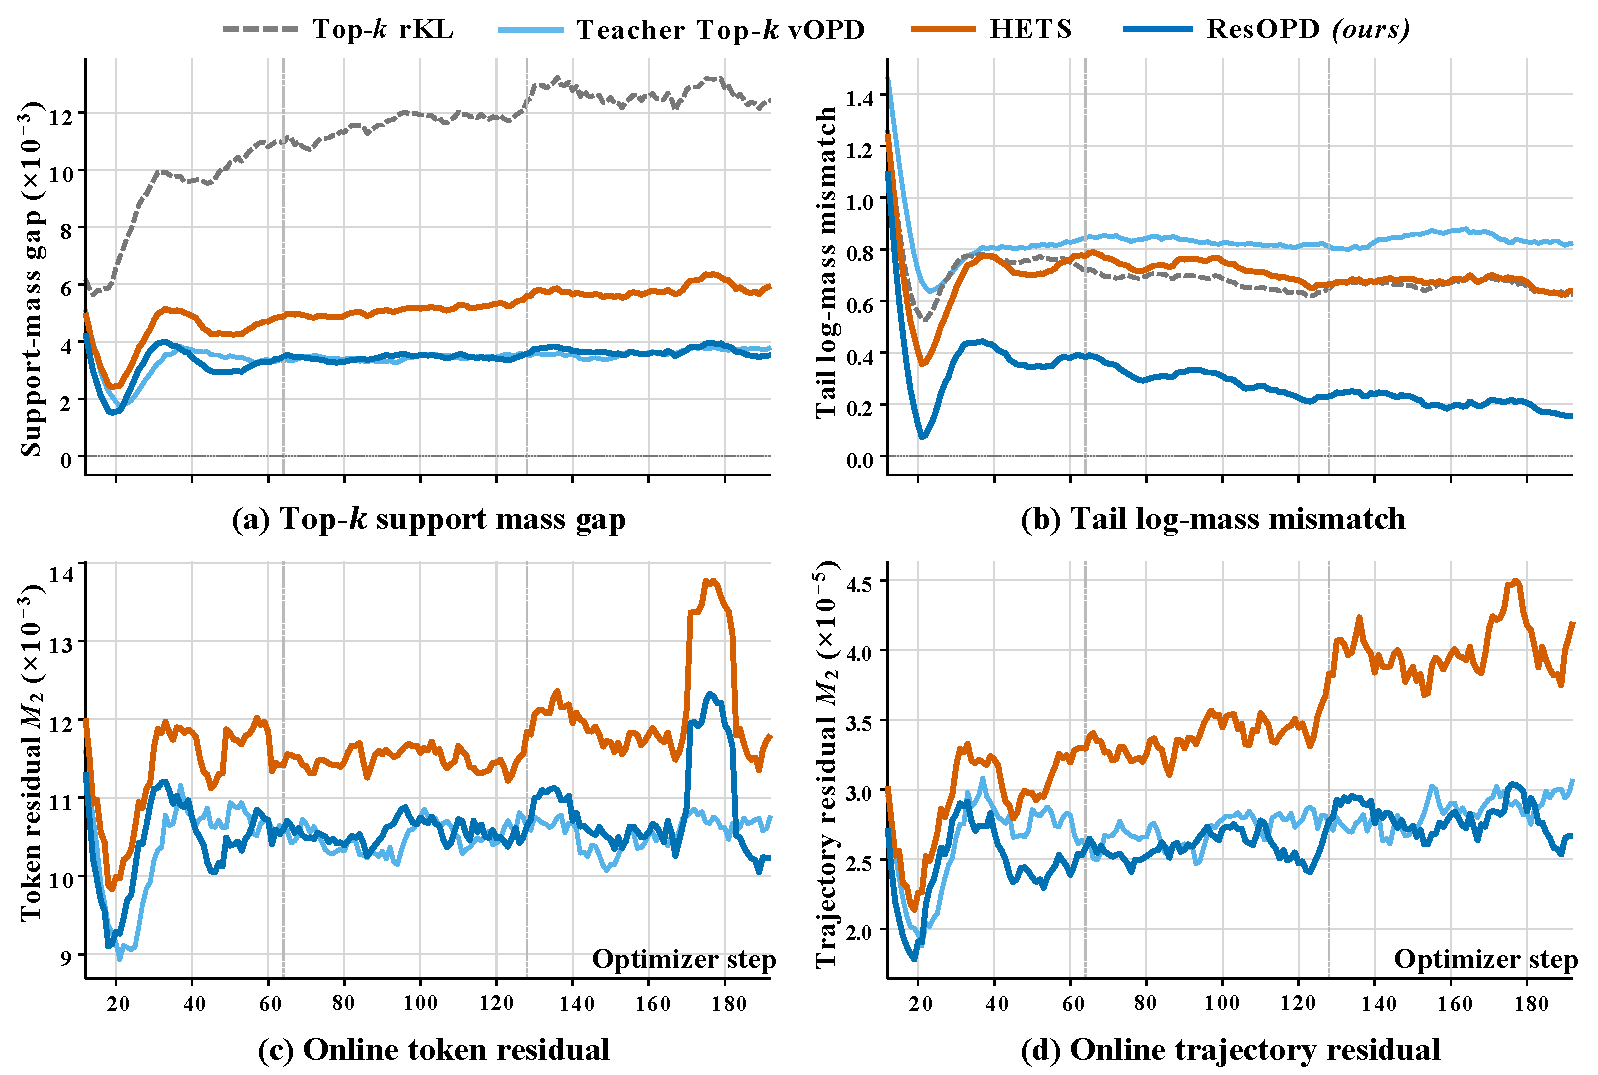
\includegraphics[width=0.85\textwidth]{figs/math_dynamics_v10.pdf}
\caption{\textbf{Training-time diagnostics} (64 steps/epoch; lower is better).
\textbf{Panels (a) and (b)} illustrate the student--teacher mismatch in Top-$k$ support mass and tail log-mass across vOPD, HETS, ResOPD, and direct Teacher Top-$k$ rKL.
\textbf{Panels (c) and (d)} compare vOPD, HETS and ResOPD via the squared residual between the binary Top-$k$ indicator and its student-predicted probability, evaluated at the token level and trajectory level, respectively. Detailed formulations are provided in Appendix~\ref{app:online-residual-moments}.}
\label{fig:training-dynamics-event-g0}
\vspace{-6mm}
\end{figure}

As illustrated in Tab.~\ref{tab:stable-dynamics} and Fig.~\ref{fig:training-dynamics-event-g0}, \method{} consistently suppresses both student--teacher mass discrepancies and stochastic residual fluctuations relative to HETS on average over 192 training steps. Across the matched HETS--\method{} runs, \method{} reduces the support-mass gap by $32.3\%$ and the tail log-mass mismatch by $55.5\%$.
Although Teacher-Top-$k$ vOPD exhibits a comparable support-event $M_2$, this scalar residual on self-generated trajectories omits centered log-ratio and score geometry, and exact gradient covariance comparisons on shared frozen prefixes (Tab.~\ref{tab:mechanism}) confirm ResOPD's structural advantage.

This provides a mechanistic explanation for the optimization behavior of \method{}. Under HETS, the full fine-tail gradient correction is concentrated on rare tail-hit events. Despite approximately $98.4\%$ head coverage, a $30\text{K}$-token reasoning trace still contains 460--470 such corrections, accumulating to thousands per optimizer step. By subtracting the payload-available tail-bucket component $\bmean_B$, \method{} redistributes the predictable between-event component while preserving the full-rKL expectation under the on-policy condition in Sec.~\ref{subsec:evidence}. Downstream accuracy remains noisier because it depends on discrete answer correctness, but the completion-only Teacher NLL audit below shows consistently higher teacher likelihood of student-generated trajectories for \method{}. Together with the matched endpoint and curve-AUC results, these diagnostics connect the estimator-level covariance reduction to a smoother optimization path and improved downstream performance.

\vspace{-4mm}
\subsubsection{Behavioral fidelity}
\label{sec:math-eval-diagnostics}

Beyond task-specific accuracy metrics (e.g., avg@2 and avg@16 on downstream math benchmarks), monitoring the student's negative log-likelihood under the teacher model provides an intrinsic, task-agnostic readout of distillation fidelity. Specifically, a lower Teacher NLL indicates that the student samples receive higher likelihood under the teacher.

Fig.~\ref{fig:teacher-nll} tracks this metric across the matched Math run. As illustrated in Panel~A, while both estimators begin around $0.46$\,nats/token, ResOPD achieves a steeper drop by step 6 and sustains a monotonic decline down to $0.36$\,nats/token by step 192. In contrast, HETS plateaus around $0.385$\,nats/token and displays slight drift in later stages. The difference $\Delta\text{Teacher-NLL (ResOPD} - \text{HETS)}$ in Panel~B remains strictly negative across all optimizer steps, widening to over $-0.027$\,nats/token. This demonstrates that ResOPD consistently preserves higher behavioral fidelity to the teacher than HETS, offering evidence of higher teacher-likeness, complementary to accuracy.

% \begin{figure}[htbp]
% \centering
% 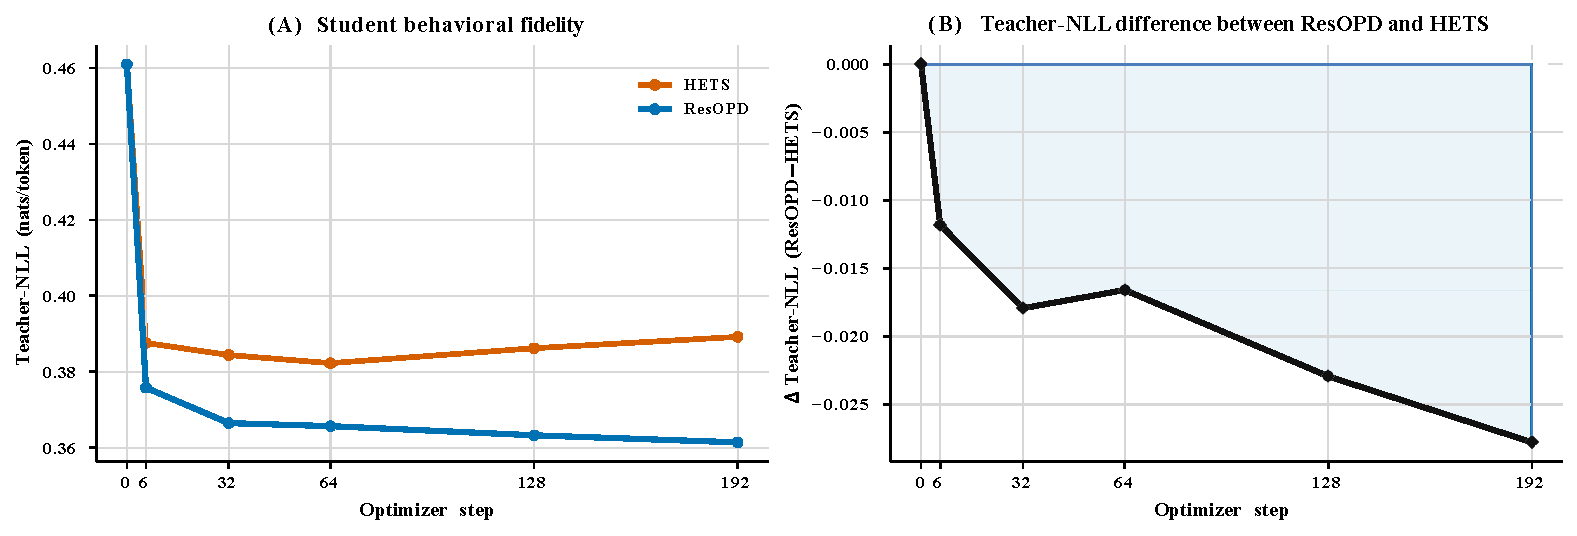
\includegraphics[width=0.85\textwidth]{figs/teacher_nll_fidelity_v3.pdf}
% \vspace{-2mm}
% \caption{\textbf{Teacher negative log-likelihood (NLL) across training in the Math OPD setup.}
% Evaluations are computed over the four core benchmark families with identical weights to the main suite: AIME26, HMMT26, DeepMath held-out, and OlymMATH. Lower values indicate higher fidelity to the Teacher distribution.}
% \label{fig:teacher-nll}
% \end{figure}

\subsection{Cross-domain transfer to science and coding}
\label{sec:cross-domain}

\begin{figure}[htbp]
\centering
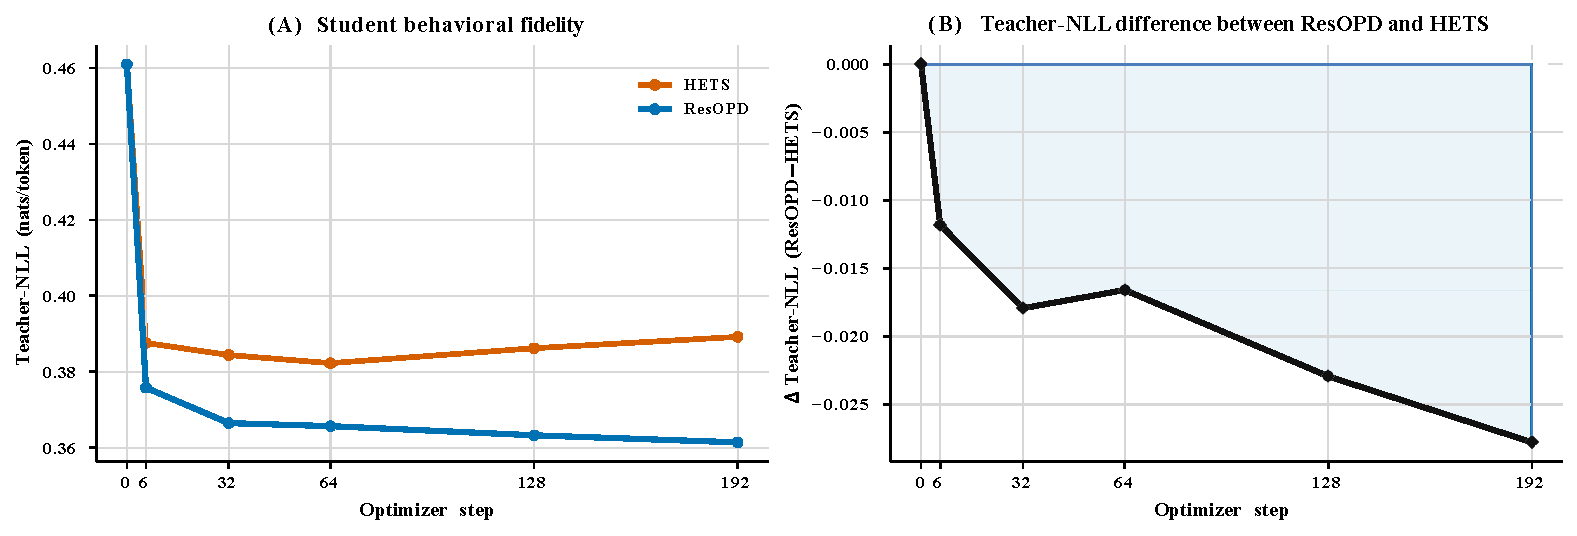
\includegraphics[width=0.9\textwidth]{figs/teacher_nll_fidelity_v3.pdf}
\vspace{-2mm}
\caption{\textbf{Teacher negative log-likelihood (NLL) across training in the Math OPD setup.}
Evaluations are computed over the four core benchmark families with identical weights to the main suite: AIME26, HMMT26, DeepMath held-out, and OlymMATH. Lower values indicate higher fidelity to the Teacher distribution.}
\label{fig:teacher-nll}
\end{figure}

\begin{table}[h]
\caption{
Distillation results from Qwen3-30B-A3B-Instruct to Qwen3-4B. Evaluations use avg@10 for GPQA-D and avg@3 for SuperGPQA, LCB-v5, and LCB-v6.
AUC integrates performance across the fixed training trajectory (Base/10/25/50/100).
}
\label{tab:qwen3-transfer}
\centering
\small
\setlength{\tabcolsep}{3.5pt}
\renewcommand{\arraystretch}{1.18}

\newcolumntype{Y}{>{\centering\arraybackslash}X}

\begin{tabularx}{\linewidth}{l YYYY YY}
\toprule
\multirow{2}{*}[-2ex]{\textbf{Method}}
& \multicolumn{2}{c}{\textbf{Science Benchmarks (\%)}}
& \multicolumn{2}{c}{\textbf{Code Benchmarks (\%)}}
& \multicolumn{2}{c}{\textbf{Aggregate (\%)}} \\
\cmidrule(lr){2-3} \cmidrule(lr){4-5} \cmidrule(l){6-7}
& \shortstack{GPQA-D\\{\scriptsize(avg@10)}}
& \shortstack{SuperGPQA\\{\scriptsize(avg@3)}}
& \shortstack{LCB-v5\\{\scriptsize(avg@3)}}
& \shortstack{LCB-v6\\{\scriptsize(avg@3)}}
& \shortstack{Avg.\\Score}
& \shortstack{Avg.\\AUC} \\
\midrule

\rowcolor{gray!18}\multicolumn{7}{@{}l}{\textit{\textbf{$\blacktriangledown$ Original Models}}} \\
Student             & 45.25          & 32.46          & 21.76          & 24.38          & 30.96          & -- \\
Teacher             & 56.06          & 48.87          & 45.51          & 41.71          & 48.04          & -- \\

\midrule
\rowcolor{gray!18}\multicolumn{7}{@{}l}{\textit{\textbf{$\blacktriangledown$ Unbiased rKL Estimators}}} \\
Sampled-token OPD   & \textbf{50.30} & \underline{36.87} & 43.31          & 39.43          & 42.48          & 41.21 \\
HETS                & \underline{48.89} & 36.10          & \underline{46.31} & \textbf{43.24} & \underline{43.63} & \underline{42.13} \\

\rowcolor{lineblue!15}
\textbf{ResOPD} (\textit{ours}) & 47.12          & \textbf{37.54} & \textbf{48.90} & \underline{43.05} & \textbf{44.15} & \textbf{42.65} \\
\bottomrule
\end{tabularx}
\end{table}

To further evaluate the generalization and cross-domain effectiveness of ResOPD, we follow \citet{heo2026policy} and extend our investigation to science and coding tasks. Our experimental protocol largely mirrors that of \citet{heo2026policy}: we distill from a Qwen3-30B-A3B-Instruct \citep{yang2025qwen3} teacher into a Qwen3-4B student, training on a 30k-sample mixture compiled from OpenMathReasoning \citep{moshkov2025aimo}, OpenScienceReasoning-2 \citep{nvidia2025opensciencereasoning2}, and OpenCodeReasoning \citep{ahmad2025opencodereasoning}. The run uses full-support ancestral rollouts with temperature $1.0$, top-$p=1.0$, and top-$k=-1$, without thinking mode. For evaluation, we benchmark the code domain on LiveCodeBench \citep[LCB;][]{jain2025livecodebench} v5 (167 problems) and v6 (175 problems). For the science domain, we evaluate on GPQA-Diamond \citep[GPQA-D, 198 problems;][]{rein2023gpqa} and SuperGPQA \citep{du2026supergpqa}, adopting the exact 650-problem subset used in \citet{heo2026policy}.

Tab.~\ref{tab:qwen3-transfer} reports the evaluation results. Overall, ResOPD achieves the strongest aggregate results, leading in both terminal average score ($44.15\%$) and trajectory AUC ($42.65\%$). Although ResOPD and HETS nominally surpass the teacher on code tasks (e.g., ResOPD's $48.90\%$ vs.\ $45.51\%$ on LCB-v5), paired bootstrap 95\% CIs cross zero (e.g., ResOPD$-$Teacher spans $[-2.48, +5.33]$ on LCB-v6), indicating on-par performance rather than statistically significant super-teacher generalization.
Across training scales, ResOPD maintains consistent optimization advantages (e.g., reducing trajectory residual $M_2$ by $9.5\%$--$12.6\%$ and gradient norms by $14.6\%$--$23.7\%$) and exhibits directional AUC gains over HETS on code ($+0.48$ and $+0.73$ points), even though Sampled-token OPD yields the strongest performance on science tasks (detailed training checkpoint curves are provided in Appendix~\ref{app:cross-qwen3}).
\vspace{-2mm}

\subsection{Online support-size ablation}
\label{sec:online-support}

\begin{table}[t]
\caption{Performance under different Top-$k$ support sizes (matched one-epoch budget). Evaluation setups follow Tab.~\ref{tab:math-terminal} (avg@16 for AIME26/HMMT26 and avg@2 for OlymMATH). $\Delta$ denotes the average improvement of ResOPD over HETS.}
\label{tab:topk-breakdown}
\centering
\small
\renewcommand{\arraystretch}{1.1}

\begin{tabular*}{0.80\textwidth}{@{\extracolsep{\fill}}cc cccc c@{}}
\toprule
\textbf{$k$} & \textbf{Method} & \textbf{AIME26} & \textbf{HMMT26} & \textbf{OlymMATH} & \textbf{Average} & \textbf{$\Delta$} \\
\midrule
\multirow{2}{*}{1}
& HETS & \textbf{60.62} & 37.69          & 34.75          & 44.35          & \multirow{2}{*}{$+0.11$} \\
& ResOPD  & 56.88          & \textbf{39.02} & \textbf{37.50} & \textbf{44.47} & \\
\addlinespace[3pt]
\multirow{2}{*}{4}
& HETS & 59.17          & 36.93          & 34.50          & 43.53          & \multirow{2}{*}{$+1.01$} \\
& ResOPD  & \textbf{60.00} & \textbf{37.88} & \textbf{35.75} & \textbf{44.54} & \\
\addlinespace[3pt]
\multirow{2}{*}{16}
& HETS & 57.92          & \textbf{39.39} & 35.75          & 44.35          & \multirow{2}{*}{$+0.70$} \\
& ResOPD  & \textbf{59.38} & 39.02          & \textbf{36.75} & \textbf{45.05} & \\
\addlinespace[3pt]
\multirow{2}{*}{32}
& HETS & 59.79          & \textbf{39.02} & 36.75          & 45.19          & \multirow{2}{*}{$+1.56$} \\
& ResOPD  & \textbf{61.67} & 38.07          & \textbf{40.50} & \textbf{46.75} & \\
\bottomrule
\end{tabular*}
\end{table}

\begin{figure}[t]
\centering
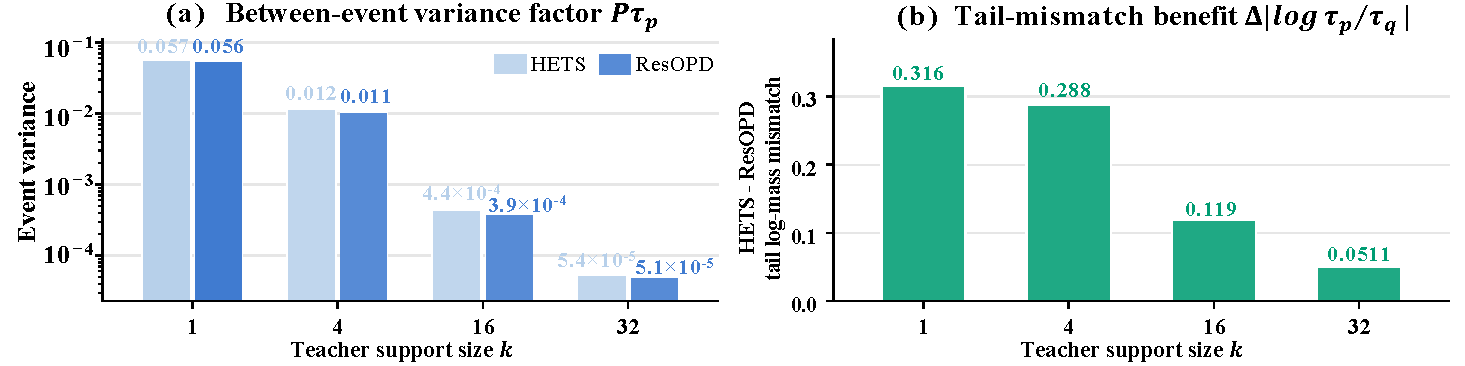
\includegraphics[width=0.9\textwidth]{figs/topk_ablation_v10.pdf}
\caption{Online diagnostic metrics across teacher Top-$k$ support sizes.
\textbf{(a)} Between-event variance factor $P\tau_p$ for HETS and ResOPD, characterizing the scaling coefficient of the head-versus-tail partition.
\textbf{(b)} Tail log-mass mismatch reduction ($\text{HETS} - \text{ResOPD}$, measured via $\Delta|\log(\tau_p / \tau_q)|$).}
\label{fig:topk-ablation}
\vspace{-4mm}
\end{figure}

Appendix~\ref{app:fixed-prefix-sweep} examines the impact of the support size $k$ with frozen prefixes, reporting the exact covariance trace and NSR. In contrast, here we provide an end-to-end online ablation of OPD. Specifically, Tab.~\ref{tab:topk-breakdown} and Fig.~\ref{fig:topk-ablation} show the results across teacher support sizes $k \in \{1, 4, 16, 32\}$.
As shown in Tab.~\ref{tab:topk-breakdown}, ResOPD consistently outperforms HETS across all tested support sizes in average downstream accuracy, with improvements ranging from $+0.11$ percentage points at $k=1$ up to $+1.56$ points at $k=32$.
However, while downstream task scores consistently favor ResOPD, the intrinsic variance reduction benefit offered by ResOPD is expected to diminish as $k$ increases, since a larger teacher support naturally captures more probability mass and renders tail corrections less frequent.

Fig.~\ref{fig:topk-ablation} validates this mechanism on the runs from Tab.~\ref{tab:topk-breakdown}.
In Fig.~\ref{fig:topk-ablation}(a), HETS and ResOPD exhibit nearly identical variance factors $P\tau_p$,  both dropping by over three orders of magnitude from $k=1$ to $32$. This directly scales the theoretical
ResOPD--HETS variance contrast alongside tail-mean approximation quality.
Meanwhile, Fig.~\ref{fig:topk-ablation}(b) shows that ResOPD consistently lowers tail log-mass mismatch across all supports,
with the largest margin in tight-support regimes.

\subsection{Rollout sampling: default filters versus full support}
\label{sec:rollout-ablation}
While the idealized ancestral sampling condition $A\sim p_\theta$ is strictly enforced in both our exact enumeration audits (Sec.~\ref{sec:exact-audit}) and the cross-domain transfer experiments (Sec.~\ref{sec:cross-domain}), we also verify for completeness that the primary math results do not depend on rollout truncation. Specifically, we evaluate the first training epoch under full-support sampling ($\text{top-}p=1.0$, $\text{top-}k=-1$) while keeping all other training hyperparameters identical.
As shown in Tab.~\ref{tab:full-support-first-epoch}, removing the rollout filters lowers AUC for all three evaluated methods. Nevertheless, ResOPD consistently maintains its advantage over HETS and the naive baseline across both benchmark accuracy and trajectory AUC. In addition, we observe that removing rollout filters yields longer reasoning trajectories and a higher frequency of hitting the response token limit during training.

% \begin{table}[t]
% \centering
% \small
% \caption{\textbf{First-epoch Math performance under default vs. full-support rollouts.}
% Benchmark scores and Avg. denote step-64 accuracy (\%); $\text{AUC}$ (\%) measures the normalized learning curve area over steps $\{0, 6, 32, 64\}$.
% \textit{Default}: top-$p=0.95$, top-$k=20$; \textit{Full}: top-$p=1.0$, top-$k=-1$.}
% \vspace{-2mm}
% \label{tab:full-support-first-epoch}
% \setlength{\tabcolsep}{5pt}
% \renewcommand{\arraystretch}{1.15}
% \begin{tabular}{llcccccc}
% \toprule
% \textbf{Rollout} & \textbf{Method} & \textbf{DeepMath} & \textbf{AIME26} & \textbf{HMMT26} & \textbf{OlymMATH} & \textbf{Avg.} & \textbf{AUC} \\
% \midrule
% \multirow{3}{*}{Default}
% & Naive Top-$k$ rKL & 53.17 & 56.04 & 35.42 & 35.00 & 44.91 & 45.45 \\
% & HETS              & 53.17 & 59.17 & 36.93 & 34.50 & 45.94 & 46.12 \\
% & ResOPD            & \textbf{54.76} & \textbf{60.00} & \textbf{37.88} & \textbf{35.75} & \textbf{47.10} & \textbf{47.57} \\
% \midrule
% \multirow{3}{*}{Full}
% & Naive Top-$k$ rKL & 45.44 & 55.42 & 35.80 & 34.25 & 42.72 & 44.96 \\
% & HETS              & 49.80 & 57.50 & \textbf{37.88} & 35.50 & 45.17 & 45.68 \\
% & ResOPD            & \textbf{57.14} & \textbf{60.42} & \textbf{37.88} & \textbf{36.00} & \textbf{47.86} & \textbf{46.79} \\
% \bottomrule
% \end{tabular}
% \end{table}

\subsection{Learning-rate sensitivity}
\label{sec:lr-sensitivity}

\begin{table}[t]
\centering
\small
\caption{\textbf{First-epoch Math performance under default vs. full-support rollouts.}
Benchmark scores and Avg. denote step-64 accuracy (\%); $\text{AUC}$ (\%) measures the normalized learning curve area over steps $\{0, 6, 32, 64\}$.
\textit{Default}: top-$p=0.95$, top-$k=20$; \textit{Full}: top-$p=1.0$, top-$k=-1$.}
\vspace{-2mm}
\label{tab:full-support-first-epoch}
\setlength{\tabcolsep}{5pt}
\renewcommand{\arraystretch}{1.15}
\begin{tabular}{llcccccc}
\toprule
\textbf{Rollout} & \textbf{Method} & \textbf{DeepMath} & \textbf{AIME26} & \textbf{HMMT26} & \textbf{OlymMATH} & \textbf{Avg.} & \textbf{AUC} \\
\midrule
\multirow{3}{*}{Default}
& Naive Top-$k$ rKL & 53.17 & 56.04 & 35.42 & 35.00 & 44.91 & 45.45 \\
& HETS              & 53.17 & 59.17 & 36.93 & 34.50 & 45.94 & 46.12 \\
& ResOPD            & \textbf{54.76} & \textbf{60.00} & \textbf{37.88} & \textbf{35.75} & \textbf{47.10} & \textbf{47.57} \\
\midrule
\multirow{3}{*}{Full}
& Naive Top-$k$ rKL & 45.44 & 55.42 & 35.80 & 34.25 & 42.72 & 44.96 \\
& HETS              & 49.80 & 57.50 & \textbf{37.88} & 35.50 & 45.17 & 45.68 \\
& ResOPD            & \textbf{57.14} & \textbf{60.42} & \textbf{37.88} & \textbf{36.00} & \textbf{47.86} & \textbf{46.79} \\
\bottomrule
\end{tabular}
\end{table}

\paragraph{Experimental setup and evaluation protocol.}
To evaluate optimization robustness under aggressive step sizes, we conduct a controlled learning-rate sweep ($k=4$) identical to the primary Math experimental setup, except that training is compressed to 1~epoch (64 optimizer steps). All runs share a batch size of 16, a 32K response budget, and identical sampling configurations with the primary experiments. Checkpoints at steps 0, 6, 32, and 64 are evaluated under the Macro-4 protocol (averaging 16 responses per problem for AIME26 and HMMT26, and 2 responses for DeepMath held-out and OlymMATH).
\vspace{-4mm}

\begin{table}[t]
\centering
\small
\caption{\textbf{Learning-rate sensitivity of HETS vs.\ ResOPD.} $\Delta$ denotes the improvement of ResOPD over HETS.}
\vspace{-2mm}
\label{tab:lr-sensitivity}
\renewcommand{\arraystretch}{1.18}
\setlength{\tabcolsep}{7pt}
\begin{tabular}{@{}l cc c cc c@{}}
\toprule
\multirow{2}{*}{\textbf{Learning Rate}}
& \multicolumn{3}{c}{\textbf{Final Score (\%)}}
& \multicolumn{3}{c}{\textbf{Trajectory AUC (\%)}} \\
\cmidrule(lr){2-4} \cmidrule(l){5-7}
& HETS & ResOPD & $\Delta$
& HETS & ResOPD & $\Delta$ \\
\midrule
$1\times10^{-6}$ & 45.94 & \textbf{47.10} & $+1.16$ & 46.12 & \textbf{47.57} & $+1.45$ \\
$2\times10^{-6}$ & 45.94 & \textbf{46.61} & $+0.67$ & 45.69 & \textbf{46.17} & $+0.48$ \\
$5\times10^{-6}$ & 42.54 & \textbf{46.35} & \textbf{+3.81} & 43.88 & \textbf{47.77} & \textbf{+3.89} \\
\bottomrule
\end{tabular}
\vspace{-4mm}
\end{table}

\paragraph{Performance resilience across learning rates.}
As shown in Tab.~\ref{tab:lr-sensitivity}, ResOPD demonstrates substantially stronger resilience at elevated learning rates. When scaling the learning rate to $5\times10^{-6}$, HETS suffers severe degradation, with its final score dropping from $45.94\%$ to $42.54\%$ ($-3.40\%$) and its trajectory AUC declining by $2.24\%$. In contrast, ResOPD retains consistent performance ($46.35\%$ final score, $47.77\%$ AUC), widening its lead over HETS to $+3.81\%$ in final score and $+3.89\%$ in AUC.
Examining the sub-benchmark breakdown at this aggressive rate, ResOPD's advantage is consistently positive across all four constituent benchmarks at step 64: $+3.96\%$ on AIME26, $+2.08\%$ on HMMT26, $+6.94\%$ on DeepMath held-out, and $+2.25\%$ on OlymMATH. We provide detailed training dynamics across different learning rates in Appendix~\ref{app:lr-sensitivity}.
\vspace{-4mm}

\paragraph{Stability boundaries and failure modes.}
When the learning rate is scaled further to $1\times10^{-5}$, both methods diverge rapidly, triggering heavy gradient clipping ($4/6$ steps for HETS and $5/6$ steps for ResOPD) and severe response-length collapse within six optimizer steps. While ResOPD does not shift the ultimate divergence boundary ($1\times10^{-5}$) under our default training recipe, its coarse-tail residualization provides a substantially wider stability margin in moderately aggressive regimes. Scaling beyond this threshold may require coordinating higher learning rates with complementary stabilization techniques (such as larger batch sizes or tighter clipping thresholds), which we leave to future work.
\vspace{-4mm}

\subsection{Comparing the two-control endpoints}
\label{sec:control-comparison}

The analysis in Sec.~\ref{sec:unified} identifies a distinct opportunity to
reduce within-tail variance through $\gamma$. We evaluate that prediction
using SC-TA ($\gamma=1$) and ResOPD ($\gamma=0$), keeping the observable
coarse control $\bm B=\bmean_B$ fixed.

\subsubsection{Cross-distribution fixed-prefix audit}
While the two-control framework indicates that SC-TA ($\gamma=1$) can mitigate within-tail fluctuations beyond ResOPD ($\gamma=0$), Equation~(\ref{eq:event-improvement}) implies this ordering is distribution-dependent rather than universal. To evaluate stability across domains, we freeze the Qwen3.5-4B/27B pair (Top-4 support, 64-token horizon) across three natural prompt distributions (DeepMath \citep{deepmath}, MegaScience \citep{fan2025megascience} and SynLogic \citep{liu2026synlogic}), evaluating 128 trajectories (8,192 prefixes) with 20,000 bootstrap resamples. We track the normalized trace variance reduction:
\begin{equation}
  \Delta \coloneqq \frac{\mathcal{V}_{\mathrm{SC}} - \mathcal{V}_{\mathrm{ResOPD}}}{\mathcal{V}_{\mathrm{sampled}}},
\end{equation}
where negative values favor SC-TA.

As reported in Tab.~\ref{tab:scta-cross-distribution}, the aggregate trace variance consistently favors SC-TA over ResOPD across all three evaluated domains ($\Delta \in [-0.207, -0.126]$). Simultaneously, prefix-level crossover remains non-trivial (up to $18.0\%$ of prefixes favor ResOPD in SynLogic). This empirically corroborates the qualified prediction of our two-control formulation: while setting $\gamma=1$ may yield lower variance in expectation, the local variance ordering remains strictly prefix-dependent rather than globally uniform.

In principle, one could pre-select a subset of prompts from the training distribution to empirically calibrate an optimal coefficient $\gamma^\star$, potentially unlocking additional variance reduction during optimization (even though $\gamma^\star$ inherently evolves alongside model weights). In practice, however, our experiments indicate that the incremental gains from such calibration over the fixed heuristic $\gamma=1$ are marginal. We therefore omit further discussion in favor of simplicity.

\begin{table}[t]
\caption{\textbf{SC-TA vs.\ ResOPD covariance trace ordering across natural prompt distributions.}}
\vspace{-2mm}
\label{tab:scta-cross-distribution}
\centering
\small
\setlength{\tabcolsep}{6.0pt}
\begin{tabular}{@{}lccc@{}}
\toprule
Dataset & $\mathcal{V}_{\mathrm{SC}} / \mathcal{V}_{\mathrm{ResOPD}}$ & $\Delta$ & ResOPD-Lower Prefixes \\
\midrule
DeepMath    & 0.512 & $-0.126$ & \phantom{0}6.8\% \\
MegaScience & 0.532 & $-0.207$ & 11.3\% \\
SynLogic    & 0.558 & $-0.161$ & 18.0\% \\
\bottomrule
\end{tabular}
\vspace{-2mm}
\end{table}

\begin{table}[t]
\caption{\textbf{Matched evaluation curves across training updates (\%).}
Evaluated on Qwen3.5-27B-to-4B distillation across AIME26/HMMT26 (avg@16) and held-out DeepMath/OlymMATH (avg@2).}
\vspace{-2mm}
\label{tab:scta-curve}
\centering
\small
\setlength{\tabcolsep}{5.5pt}
\begin{tabular}{@{}lcccccc@{}}
\toprule
Method & Base (Step 0) & Step 6 & Step 32 & Step 64 & Step 128 & Step 192 \\
\midrule
HETS  & 42.85 & \textbf{48.86} & 45.04 & 45.94 & 46.60 & 45.72 \\
ResOPD   & 42.85 & 48.23 & \textbf{47.95} & 47.10 & 47.71 & \textbf{50.12} \\
SC-TA & 42.85 & 47.66 & 46.69 & \textbf{47.26} & \textbf{48.27} & 46.33 \\
\bottomrule
\end{tabular}
\vspace{-4mm}
\end{table}

\subsubsection{Downstream evaluation comparison}
While SC-TA halves the fixed-prefix residual covariance trace of ResOPD, this advantage does not necessarily translate into superior downstream accuracy. As shown in Tab.~\ref{tab:scta-curve},
SC-TA does not exhibit a consistent downstream advantage over ResOPD: it is slightly stronger at several intermediate checkpoints, whereas ResOPD achieves the higher terminal score, with trajectory-level AUC remaining similar.

This decoupling between gradient covariance trace and downstream performance is informative rather than contradictory. While lower estimator variance validates the two-control residualization mechanism locally, downstream benchmark accuracy reflects the global trajectory of policy updates.
Consequently, while SC-TA exhibits lower overall variance across the evaluated audit sets, ResOPD retains strong aggregate performance in this evaluated setting without explicitly subtracting the additional within-tail score fluctuation.
\vspace{-4mm}
